\chapter{State of the art}
\label{chap:stateoftheart}

\drop{T}{his} chapter aims to explain the concepts and techniques in which
Alcaudon is based on. As shown in Figure ~\ref{fig:mindmap}. the project has foundations in
distributed systems, job scheduling, library design and data processing. In the
next subsections, those concepts will be analyzed in more depth.

\begin{figure}[!h]
\begin{center}
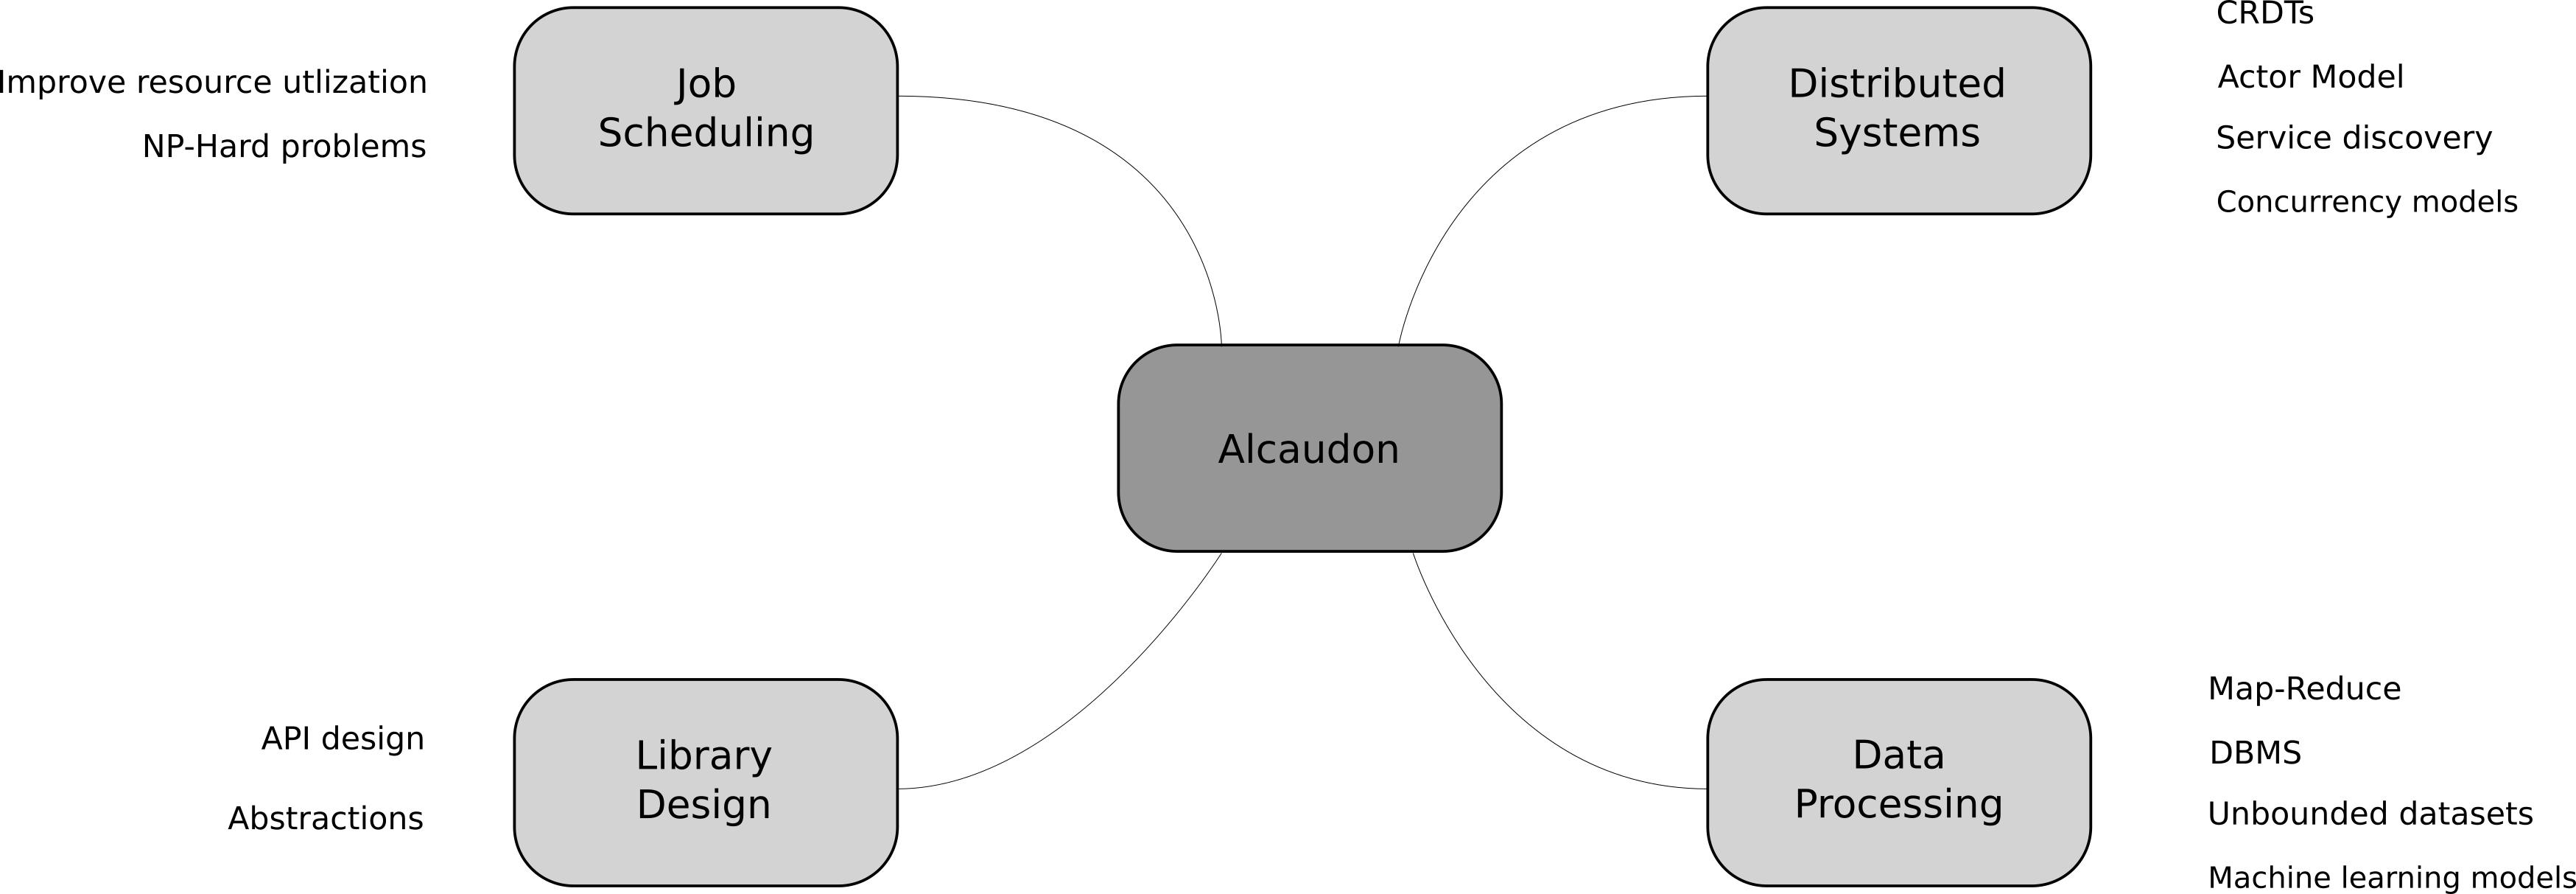
\includegraphics[width=1\textwidth]{mindmap.png}
\caption{Alcaudon foundations}
\label{fig:mindmap}
\end{center}
\end{figure}

\subsection{Data Processing}

According to a recent study by Cisco \cite{ciscosurvey}~\ref{fig:ciscodata} the
data storage is growing by 40\% yearly. That means that by 2020 datacenters will
store over 1000 ExaBytes of information. Keeping that data in silos without
performing any use of it is a poor investment.

\begin{figure}[!h]
\begin{center}
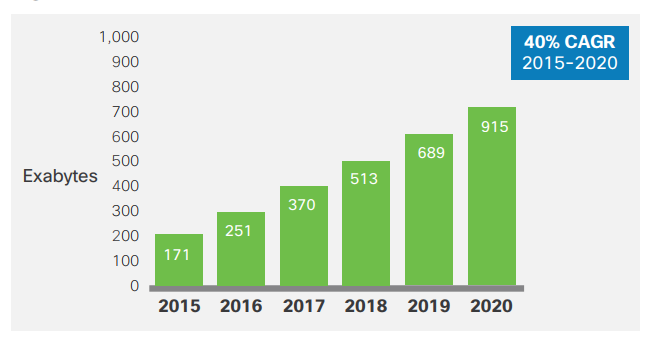
\includegraphics[width=0.8\textwidth]{ciscodata.png}
\caption{Actual Data Stored in Data Centers\cite{ciscosurvey}}
\label{fig:ciscodata}
\end{center}
\end{figure}

Processing those amounts of data using traditionals RDBMS is not practical, as they
are not designed to work with that much data. In the last years there have been
many ongoing efforts on providing tools to process and analyze large volumes of
data. Some examples could be MapReduce\cite{mapreduce}, Spark\cite{spark} and
many others. Before those frameworks appeared, there were some systems capable
of processing large amounts of data, like the supercomputers or HPC. One of the
main drawbacks of HPC is accessibility to those high end computers. Acquiring a
new Supercomputer in the event of a peak on data production is not feasible. For
companies, making an investment in a super computer is a big risk that in some
cases will not be reverted as profit.Another interesting point to make is that
Supercomputers perform well many floating-point operations per second. However,
in general the computations executed in systems like MapReduce are simple
strings manipulation, counting and so on. Given these usage patterns, it seems
that supercomputers are more suited to perform scientific analysis.

Once the limitations of HPC for \textit{big data} scenarios has been described
it is possible to explore how modern internet companies are using computing
resources to process data. For new organizations, it makes more sense to take
advantage of commodity hardware to process large amounts of data. One of the
reasons is that there are many tools to distribute data processing among large
clusters of commodity machines. Once that job is done, those machines can be
turned off or used for other purposes. Working with those systems provides
flexibility, both in resource usage and innovation capacity. 

\subsubsection{Cloud Computing}

The data processing systems described above fits very well with cloud computing
offerings such as IaaS providers.
During 2002 Amazon.com launched Amazon Web Services(AWS), one of the first cloud
providers. The idea behind AWS is to provide computing resources as a service, basically
outsourcing all the datacenter needs. The interesting part about AWS is that it provides
the needed elasticity 

TODO

List map-reduce, spark, storm

\subsection{Distributed systems}
\label{subsection:distsys}

Distributed systems can be defined as a set of computer programs, executing on
one or more computers, and coordinating actions by exchanging \textit{messages}
\cite{GuideReliable}. Those computers are usually located in a \textit{computer
  network}, a collection of computers interconnected by hardware that supports
message passing and implement routing protocols. But if this definition is taken
to the extreme, a modern multi-core processor can be characterized as a
distributed system, with many components exchanging information in a network and
coordinating actions to get work done. To some extent, it's possible to see
distributed systems as a super set of concurrent systems.

A more common example of a distributed system it is a user requesting a web page to
a server with his smartphone. This example is a typical \textit{client-server}
model. This \textit{simple} action involves the interaction of various services
such as DNS servers, load balancers, HTTP proxies and HTTP servers. All these
services use a network as a mean to interchange messages as shown in figure
~\ref{fig:client-server}.

\begin{figure}[!h]
\begin{center}
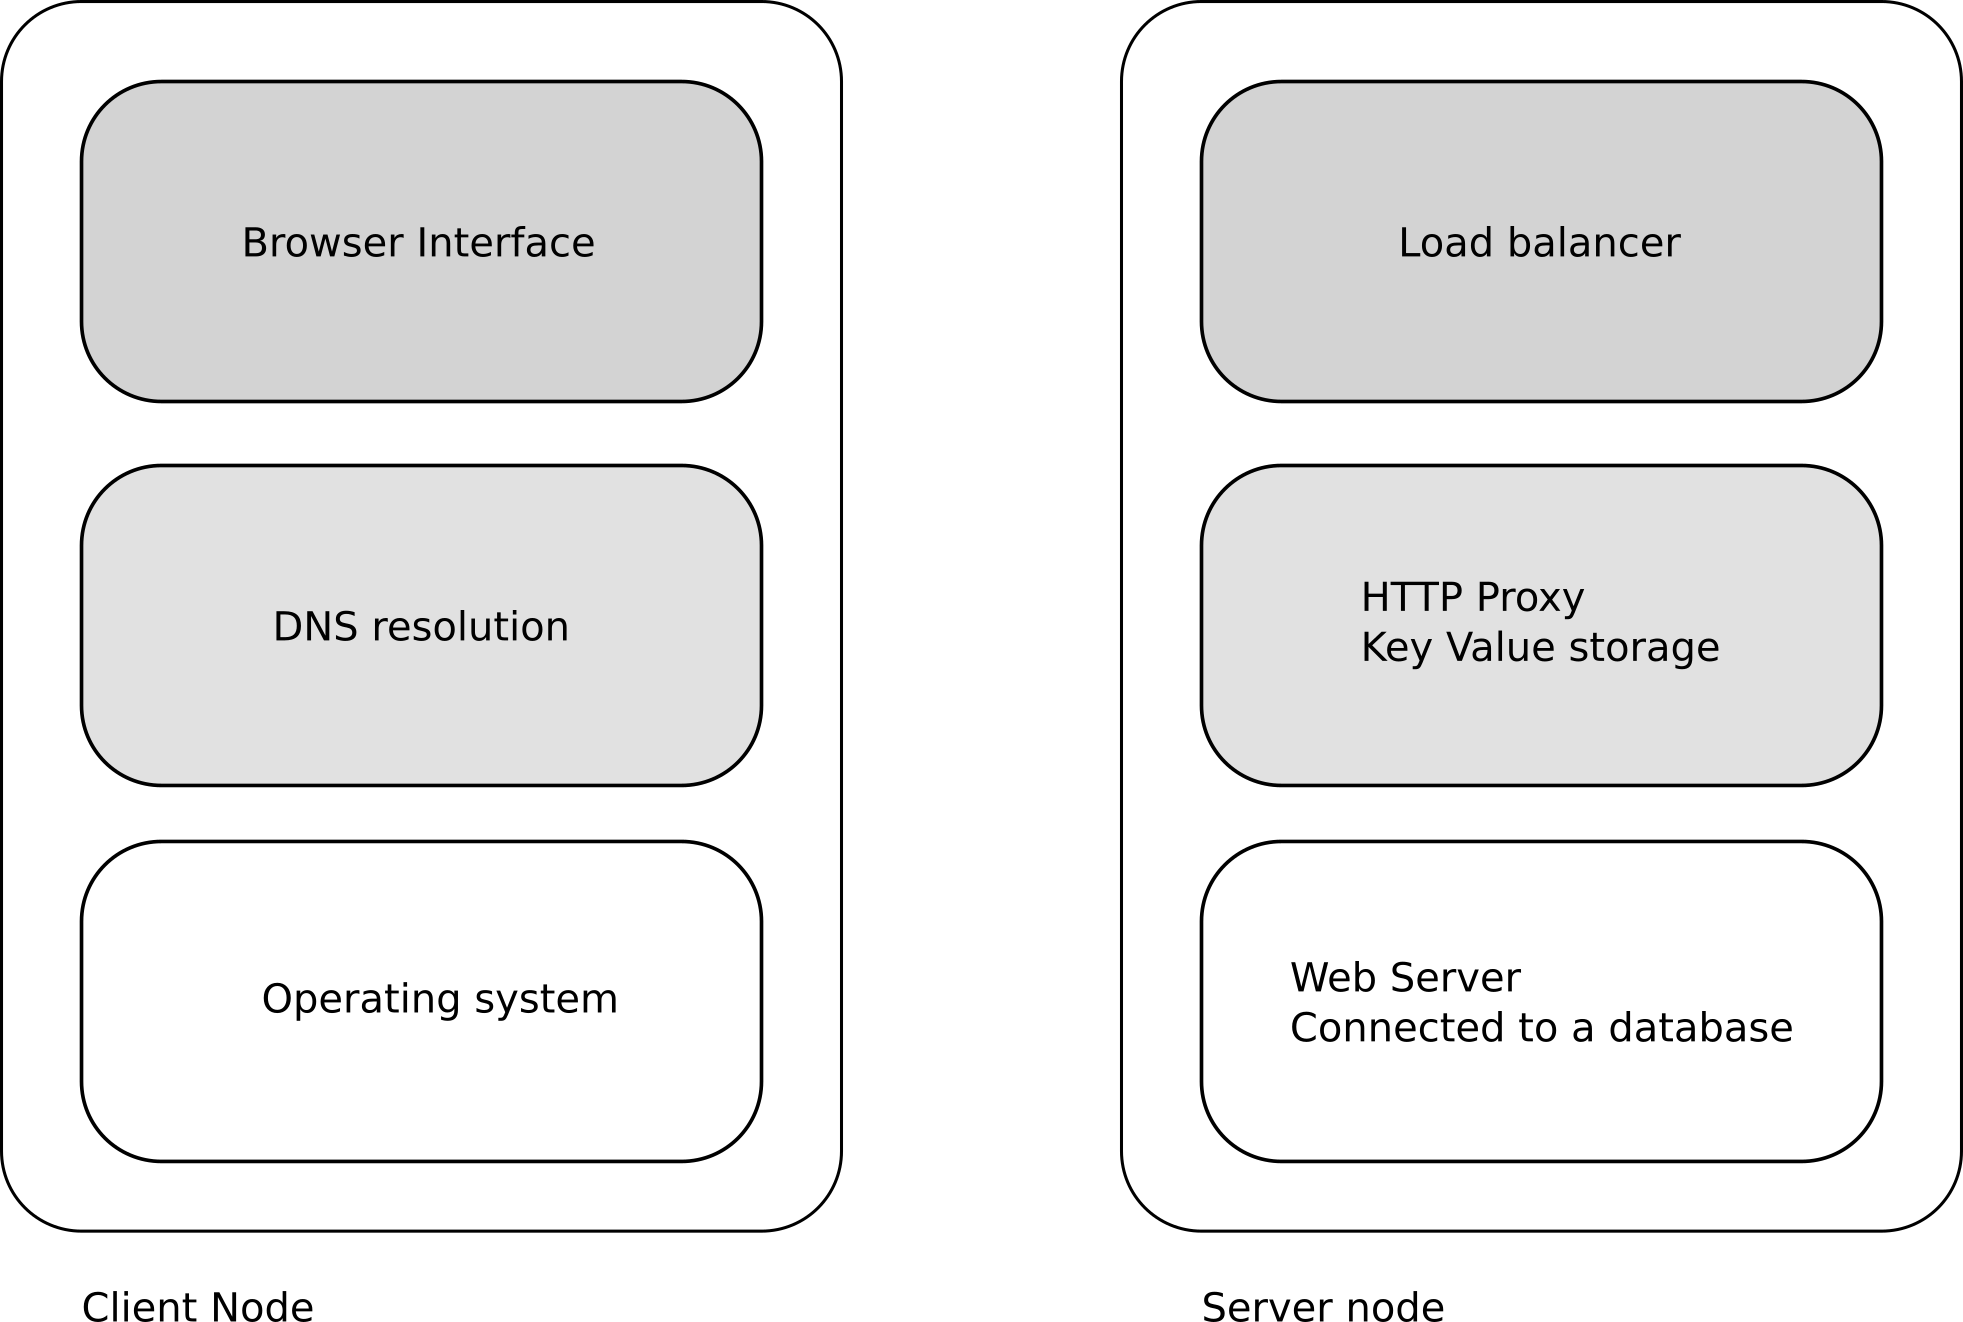
\includegraphics[width=0.7\textwidth]{client-server.png}
\caption{Client-server architecture}
\label{fig:client-server}
\end{center}
\end{figure}

As it has been previously discussed, distributed systems are very common
nowadays. They are present in fields like database systems, internet of things,
data processing and many more.

There are some reasons that make more convenient to work with distributed
systems, but the main reason is ability to scale. As defined in \cite{cloudadmin}
\begin{quote}
  A system's ability to scale is its ability to process a growing workload,
  usually measured in transactions per second, amount of data or number of
  users.
\end{quote}

Distributed programming can help designing systems with the ability to scale given
the following properties:

\begin{figure}[!h]
\begin{center}
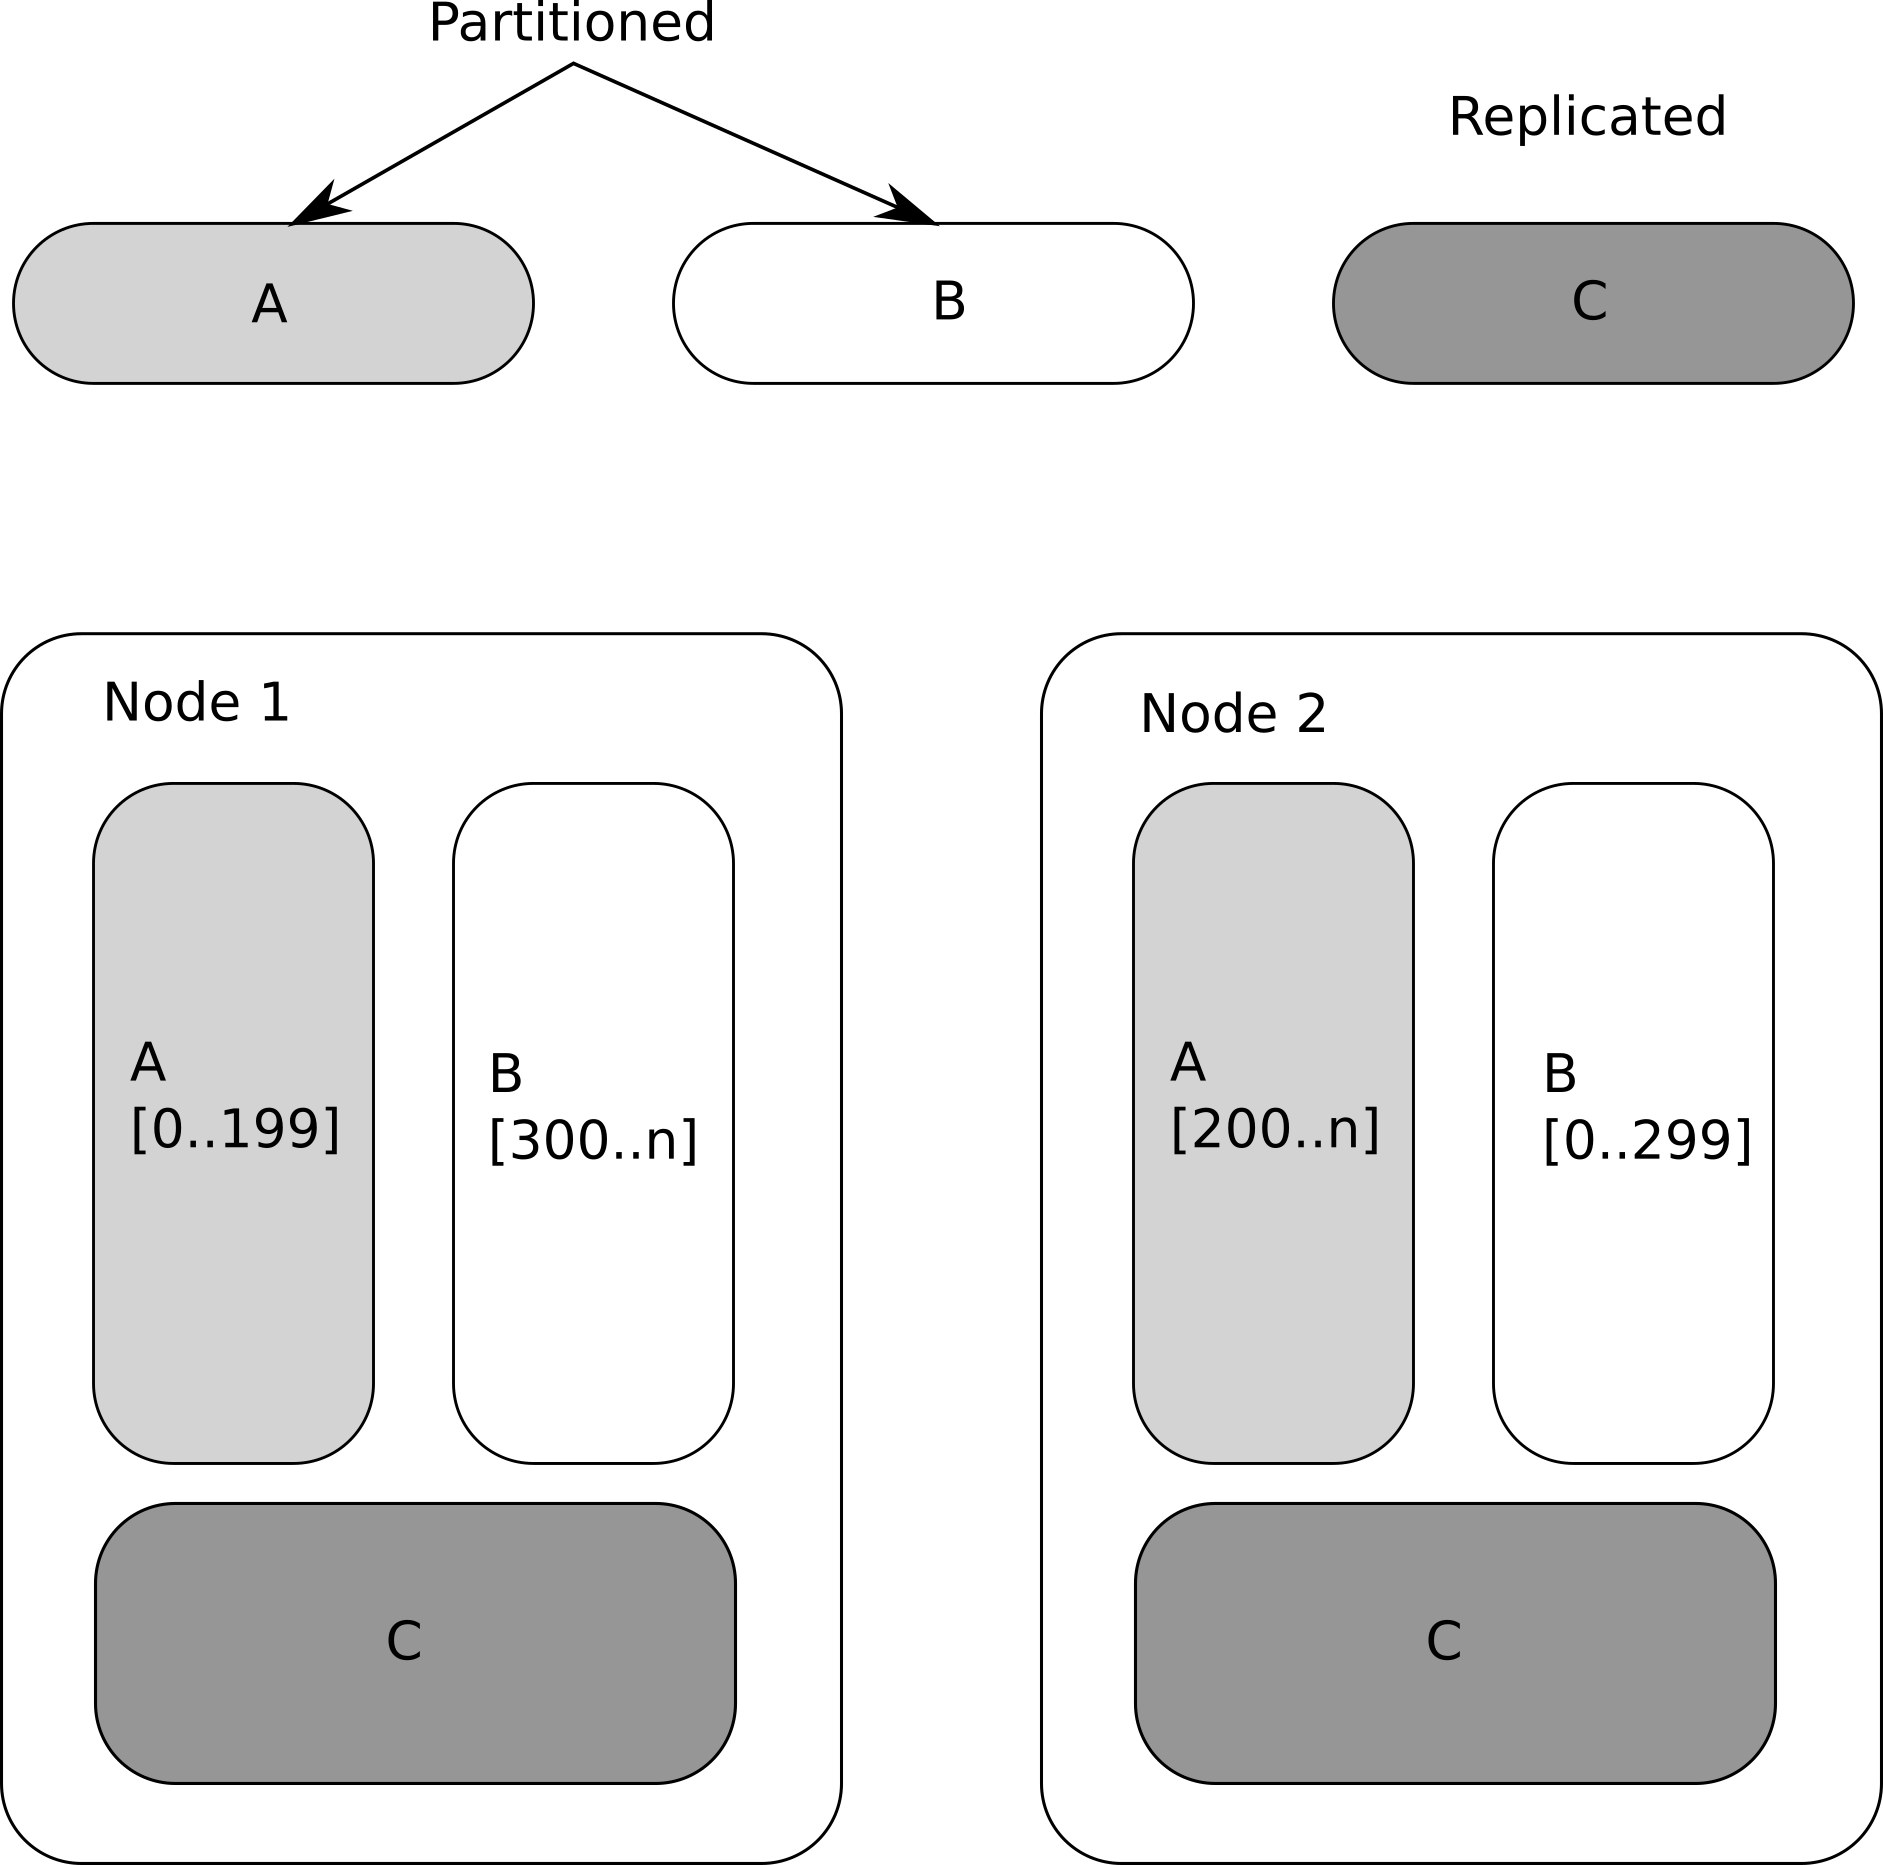
\includegraphics[width=0.7\textwidth]{partition-rep.png}
\caption{Partitioning and Replication}
\label{fig:partitioning}
\end{center}
\end{figure}

\begin{itemize}
\item \textit{Reliability}: Achieved by \textit{replication} and/or
  \textit{partitioning} as illustrated in Figure ~\ref{fig:partitioning}.
\item \textit{Elasticity}: Since the systems are designed to work in
  coordination with other processes, it is possible to add more resources to
  handle increasing workloads. But there is an upper limit imposed by the
  coordination model used.
\item \textit{Parallelism}: This is a natural outcome of having multiple resources, they
  can get work done in parallel.
\item \textit{Price/performance ratio}: Scaling vertically (using more powerful
  compute nodes), has upper limits both in available technology and in costs. As
  shown in Figure ~\ref{fig:highend} the performance gap between a high end
  server and a cluster of commodity hardware nodes is tolerable. Another factor
  to take into account when distributed systems are used is the cost of
  networking communications, as it implies an overhead in the computations.
\end{itemize}

\begin{figure}[!h]
\begin{center}
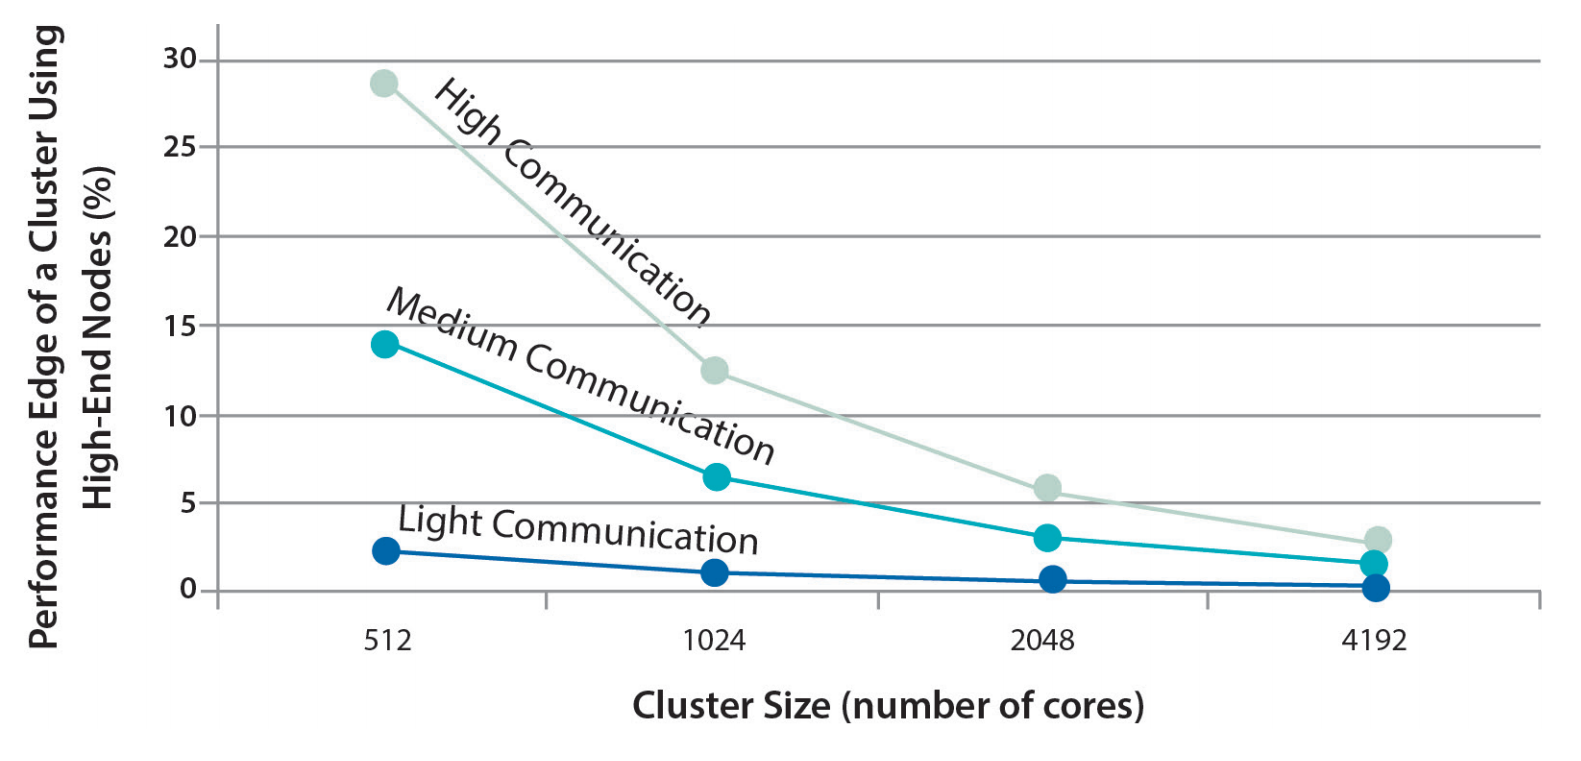
\includegraphics[width=1\textwidth]{scalingcost.png}
\caption{Performance advantage of a cluster built with large SMP server nodes
  (128-core SMP) over a cluster with the same number of processor cores built
  with low-end server nodes (four-core SMP), for clusters of varying
  size.\cite{Datacenter}}
\label{fig:highend}
\end{center}
\end{figure}

\subsubsection{Taxonomy of a distributed system}

Once described what distributed systems are and why are useful, it is possible
to define a taxonomy of distributed systems topics such as coordination
algorithms, global state collection, distributed consensus, etc.

As it can be seen the topic is wide, so for this documents only
\textit{distributed snapshots}, \textit{membership protocols} and \textit{time
  in distributed systems} will be covered.

\begin{itemize}
\item \textit{Time in distributed systems}:
  Programmers are used to think in sequential programs, where computation steps
  are executed one after the other. The reality in distributed and concurrent
  systems is quite different. Knowledge about global state among all the nodes
  in the system is likely to be outdated. A naive solution to this problem is
  use synchronization based on wall clocks but the notion of synchronized clocks
  among nodes is impractical. Protocols like NTP\cite{ntp} can have skews up to
  1000 seconds, that is unacceptable in some cases. Google makes heavy use of
  hardware-assisted time synchronization using GPS clocks and atomic clocks to
  ensure global consistency for their database Spanner\cite{180268} that can
  drift up to 100ms. Given the exposed facts, the only assumption that can be
  taken about global state, is that is partially ordered. A formal definition for
  partial order is \cite{book:lattices}:
\begin{definition}{Partial order}
  Let $P$ be a set. An order (or partial order) on $P$ is a binary relation
  $\leq$ on $P$ such that, for all $x$, $y$, $z \in P$,
  \begin{enumerate}
  \item $x \leq x$
  \item $x \leq y$ and $y \leq x$ imply $y$
  \item $x \leq y$ and $y \leq z$ imply $x \leq z$
  \end{enumerate}
\end{definition}
  Given the exposed facts, message order in distributed systems is partial. In
  environments where the message flow is unbounded the notion of completeness is
  weak, that means that there is no guarantees about when all the messages up to
  a moment $T_n$ have been received or processed. To deal with this, Alcaudon
  uses watermarks heuristics. A watermark heuristic defines that up to the
  instant $T_i$ there are high chances that all messages up to that point have
  been received. To implement these heuristics, there is a need for some global
  knowledge about latest processed events. To have that global view,
  CRDTs\cite{crdt} will be used and exposed in the following subsection.
\item \textit{Distributed snapshots}: 
  Since Alcaudon aims to be a fault-tolerant system, guarantees about persistent
  state must be enforced. To design a resilient system, persistent state
  snapshots should be taken. There are distributed algorithms to deal with this
  problem such as Lamport, bla, bla . In general, those algorithms are focused
  on taking a global state snapshot that given the constraints presented in the
  previous section is a hard problem to solve. In Alcaudon this problem is
  easier because snapshots are taken by computation. There is no need of a
  global snapshot since persistent state is local to each computation.

\item \textit{Membership protocols}: Another crucial aspect on an elastic
  distributed system is how to handle cluster membership. It is possible to
  classify them into two categories, static membership and dynamic membership.
  Static membership has a fixed list of cluster members that do not change along
  the life of the cluster. With this static membership there is a chance that at
  some point in time, some members of the cluster will not be available and
  since the cluster membership image is static, thew will be seem as accessible.
  The other approach is to use dynamic membership. It consists on having initial
  knowledge about a subset of the available nodes and later on, via gossiping
  protocols\cite{gossip} new nodes can \textit{join} the cluster. This mechanism
  handles when nodes become \textit{unavailable} as well. For Alcaudon it seems
  more suitable to adopt the latter, since one of the goals is to provide
  elasticity so the system can be scaled in the need of more computing power.
\end{itemize}

\subsubsection{CRDT}

As described before, Alcaudon needs a mechanism to keep track of the progress of
ingested events into the system. Each computation should be able to have partial
knowledge of the last watermark, and that depends on the state of a its
dependencies. One of the goals of the system is to avoid centralized
coordination as much as possible, so consensus based stores are discarded.
One available option is Convergent Replicated Data Types (CRDT)\cite{crdt}.

TODO

\subsubsection{Distributed system reliability}

Building distributed systems is not an easy task. In this subsection, different
failure scenarios that can happen in a distributed environment will be presented.

As proposed by \cite{GuideReliable}, it is possible to classify system error
causes as follows:
\begin{itemize}
\item \textit{Hardware failures}: These kind of failures are inevitable, since
  hardware have a life cycle and some components might fail.
\item \textit{Software failures}: Bugs are quite common
\item Complexity
\item Lack of failure detection
\item Hostile environments
\end{itemize}

There are costs associated with distributed programming; network latency,
fault-tolerance mechanisms and consensus can have impact in the throughput
achieved by a system. In \cite{189908} a metric named Configuration that
Outperforms a Single Thread (COST), is proposed. It measures the number of cores
needed to outperform a single threaded implementation. In this experiments,
there are many distributed processing frameworks that don't perform properly
when they are compared to a single node implementations. As a conclusion, there
are scenarios where the costs associated with distributed computing are higher
than the gains.

Alcaudon goal is to provide users a simple but powerful interface that enables
them to parallelize and distribute computations for unbounded datasets without all
the described problems.

\subsubsection{Actor Model}

To tackle all the complexity described in previous section there is a
computation model that is well suited: the actor model.

The actor model provides a high level abstraction to deal with concurrent and
distributed systems. The theoretical model was developed by Carl Hewitt in
the seventies, but it was popularized by Erlang programming language\cite{erlang}
developed by Ericsson.

It can be characterized as follows:
\begin{itemize}
\item Actors communicate via asynchronous messages
\item Actors manage their state
\item In the event of a message response they can:
  \begin{itemize}
  \item Create new child actors
  \item Send messages to another actors
  \item Stop actors (even themselves)
  \item Change their behavior for the next messages
  \end{itemize}
\end{itemize}

Since distributed systems communicate asynchronously, this model fits perfectly,
because, even in single node environments, all the computations are executed in
response to asynchronous messages. The fact that the shared state among actors
is minimal helps to tackle all the inherent complexities around concurrency.
Another interesting outcome from designing the systems using message passing is
that creating protocols come naturally in this model. The ability to change
their behavior depending on the incoming messages makes easy to model finite
state machines that fit perfectly with protocol design.

There are many implementations available\cite{wikiactor}, but the more popular
and stable versions are the Erlang programming language and Akka. Both versions
have similar features, in fact, Akka is highly inspired by Erlang. But Akka is
built on top of the JVM, and it makes it the most interesting implementation
available due to the vast ecosystem available around the JVM.

Akka have some extensions to the actor model that make it quite interesting to
build distributed systems.
\begin{itemize}
\item Actor supervision: One interesting approach of actor based design is how
  to handle failures, each actor has a supervisor that handles its life-cycle,
  exceptions included. With this supervision schema is easier to isolate failure
  scenarios into concrete actors instead of affecting the whole system. Each
  supervisor can define an strategy to apply when an child actor fails, i.e.
  restarting the actor or stopping it. This is highly beneficial because error
  handling logic is separated from business logic. These patterns resemble to
  how ships are built, where the hull is compartmentalized into different watertight
  bulkheads so if the hull is broken, the failure is limited to that bulkhead without
  compromising the ship stability. Alcaudon will benefit from this pattern to achieve
  fault-tolerant computations.
\item Logical addresses: Each actor has a virtual address based on the actor
  system and its hierarchy. This helps to provide location transparency, actors can
  change their physical location and the framework will take care of routing
  messages to the new actor location.
\item Clustering: Support for distributed actors is supported, combined with
  logical addresses make it easier to write distributed applications.
\item Persistence: Akka supports actor state persistence. It is implemented as
  an append-only log. That technique is commonly used as transaction log in
  traditional databases, each change is appended to the transaction log. In case
  of a failure, those events are applied again to the in memory database
  buffers. To avoid long recovery times, snapshots from memory are taken
  regularly so the recovery process just needs to re-apply changes from that
  point. Akka persistence is implemented as described. This feature fits very
  well to mantain Alcaudon persistent state of computations, since computations
  can be defined as actors.
\end{itemize}

In conclusion, the actor model is a good computational model to base Alcaudon
on. It have properties that allows to tackle all the presented difficulties
around writing distributed systems properly.

\subsection{Job scheduling}

Talk about NP-Problem and some state of the art schedulers.

\subsection{Library design}
